\documentclass[a4paper,11pt,oneside]{article}

% To use this template, you have to have a halfway complete LaTeX
% installation and you have to run pdflatex, followed by bibtex,
% following by one-two more pdflatex runs.
%
% Note thad usimg a spel chequer (e.g. ispell, aspell) is generolz
% a very guud ideo.
\usepackage{amsmath}
\usepackage[a4paper,top=3cm,bottom=3cm,left=3cm,right=3cm]{geometry}
\renewcommand{\familydefault}{\sfdefault}
\usepackage{helvet}
\usepackage{parskip}		%% blank lines between paragraphs, no indent
\usepackage[pdftex]{graphicx}	%% include graphics, preferrably pdf
\usepackage[pdftex]{hyperref}	%% many PDF options can be set here
\pdfadjustspacing=1		%% force LaTeX-like character spacing
\usepackage{float}
\newcommand{\myname}{Orgest Xhelili}
\newcommand{\mytitle}{Automatic Music Genre Classification using Ensemble Learning}
\newcommand{\mysupervisor}{Prof.~Dr.~Herbert~Jaeger}
\newtheorem{prop}{Proposition}

\hypersetup{
pdfauthor = {\myname},
pdftitle = {\mytitle},
pdfkeywords = {},
colorlinks = {true},
linkcolor = {blue}
}

\begin{document}
\pagenumbering{roman}

\thispagestyle{empty}

\begin{flushright}

\includegraphics[scale=0.7]{bsc-logo}
\end{flushright}
\vspace{20mm}
\begin{center}
\huge
\textbf{\mytitle}
\end{center}
\vspace*{4mm}
\begin{center}
 \Large by
\end{center}
\vspace*{4mm}
\begin{center}
\Large
\textbf{\myname}
\end{center}
\vspace*{20mm}
\begin{center}
\large
Bachelor Thesis in Computer Science
\end{center}
\vfill
\begin{flushright}
\large
\begin{tabular}{l}
\mysupervisor \\
\hline
Bachelor Thesis Supervisor \\
\\
\end{tabular}
\end{flushright}
\vspace*{8mm}
\begin{flushleft}
\large
Date of Submission: \today \\
\rule{\textwidth}{1pt}
\end{flushleft}
\begin{center}
\Large Jacobs University --- Focus Area Mobility
\end{center}

\newpage
\thispagestyle{empty}

With my signature, I certify that this thesis has been written by me
using only the indicates resources and materials. Where I have
presented data and results, the data and results are complete,
genuine, and have been obtained by me unless otherwise acknowledged;
where my results derive from computer programs, these computer
programs have been written by me unless otherwise acknowledged. I
further confirm that this thesis has not been submitted, either in
part or as a whole, for any other academic degree at this or another
institution.

\vspace{20mm}

Signature \hfill Place, Date

\newpage

\section*{Abstract}

Organizing music libraries and databases requires automatic classification of music.
Music genres are essential descriptors created by humans to label pieces of music.
This paper presents a novel approach of ensemble learning for solving the problem of 
genre classification. Ensemble learning is a machine learning paradigm where multiple 
models are trained to solve the same problem and the final result is a combination 
of the individual results by each model. Our system consists of three different classifiers:
echo state networks, support vector machines and logistic regression.

Echo state networks (ESNs) provide a supervised learning principle for analyzing and training
recurrent neural networks (RNNs). They present a more practical approach to the usage of RNNs 
because of their computational efficiency and simple implementation.\\
Support vector machines (SVMs) are supervised learning models which can be used for regression
analysis or classification problems.\\
Logistic regression is a regression model which performs linear classification by estimating 
probabilities of each of the outcomes.


\newpage
\tableofcontents

\clearpage
\pagenumbering{arabic}

\section{Introduction}
Music genres are labels created by humans to classify pieces of music giving rise to organized music libraries. 
However, the distinction between genres remains not well defined, as does their definition. 
Because of the vast amount of musical pieces, automatic genre classification is crucial for
organizing huge music databases allowing users to find the music they want to. 
Automatic genre classification is part of automatic music information retrieval where much research 
has been ongoing in the 21st century. A summary of state of the art automatic music genre 
classification may be found on this survey \cite{survey1}.

Echo state networks provide an architecture and supervised learning principle for recurrent
neural networks. They present a practical approach to training RNNs because of their simple implementation 
and computational efficiency. RNNs represent a large and varied class of computational models that are designed 
by more or less detailed analogy with biological brain modules. In an RNN numerous abstract neurons (also called units
or processing elements) are interconnected by likewise abstracted synaptic connections (or links), 
which enable activations to propagate through the network \cite{LUKO}.
ESNs differ from classic RNNs because of the usage of a fixed random reservoir
and the training of only output neurons weights \cite{spedia}. Because there are no cyclic dependencies between the trained readout connections, 
training an ESN becomes a simple linear regression task \cite{Jaeger78}.

Support vector machines are a set of supervised learning methods used for classification, regression and 
outliers detection. Given training data labeled in two classes, the SVM algorithm computes an optimal hyperplane to categorize
new data. Thus a SVM behaves as a non-probabilistic binary linear classifier. However, they can be extended to support multi 
class classification of non-linearly separable data in a probabilistic setting. 
To support non-linear classification, SVMs use the so called kernel trick, implicitly mapping their inputs into high-dimensional feature spaces. 
To support multi class classification, we use the one-vs.-one strategy, reducing a $K$ class classification problem to $K(K-1)/2$ binary classifiers.
Probabilities can be estimated for binary classification using Platt Scaling \cite{platt1999probabilistic}. For multi class
classification the probability scores can be estimated by using a pairwise coupling strategy \cite{wu2004probability}.
It should be noted that the estimation of probabilities is rather an expensive procedure.
SVMs are widely used nowadays for different machine learning problems because of their effectiveness, versatility and efficiency.

Logistic regression sometimes called the logistic model or logit model, analyzes the relationship between
multiple independent variables and a categorical dependent variable by estimating probabilities of occurrence
of an event \cite{park2013introduction}. In its classical form, logistic regression is used as a binary classifier. In this case the 
dependent variable is dichotomous. When the dependent variable is not dichotomous, a multinomial logistic
regression can be applied. 

The report is organized as follows. The second section states the motivation of this research
and describes in more detail the problem of the automatic music genre classification problem.
The third section gives a more in-depth analysis of ESNs, SVMs and logistic regression.
The fourth section documents the ensemble learning strategy used to solve the problem of automatic
music genre classification. This section also gives a summary of the state of the art and the dataset used.
The fifth section documents the evaluation criteria and the results of our experiment. The last section discusses the results and potential 
focus areas for future research in the topic.
\section{Statement and Motivation of Research}
\subsection{Music Genre Classification}
The basis of automatic music genre classification is the representation of musical pieces and the extraction
of feature vectors from the agreed representation. A symbolic representation of musical pieces is rarely available
so one has to deal with audio samples. This representation presents a good strategy as it places music genre 
classification problem in the sphere of speech recognition where more research has been done. However, using the
exact waveform of a musical piece for automatic classification is not feasible, because of the low level information 
contained in the audio samples. Therefore the first step in automatic genre classification is the extraction of useful 
features from the audio representation of musical pieces. Much work on extraction of features from music has been 
devoted to timbral texture features, rhythmic content features and pitch content features \cite{ogihara}.
\subsection{Audio Features}
\begin{itemize}
\item
Timbral texture features are used to differentiate sounds with the same pitch and loudness from each other. 
The use of timbral texture features originates from speech recognition \cite{book}. A detailed list of features used to 
characterize timbre may be found in \cite{peeters2004large}. These features are usually referred to as being low-level as they represent 
sound on samples of milliseconds. We summarize here the main low-level features used in genre classification problems as given in \cite{survey1}:
\begin{itemize}
  \item temporal features: features computed from the audio signal frame (zero-crossing rate and
   linear prediction coefficients)
  \item energy features: features that describe the energy content of the signal
  \item spectral shape features: features that describe the shape of the power spectrum
      of a signal frame: centroid, spread, skewness, kurtosis, slope, roll-off frequency, Mel-frequency cepstral
      coefficients (MFCC)
\end{itemize}
\item
Rhythmic content features are the most widely used mid-level features in audio-based music classification \cite{survey2}.
These features are used to characterize the temporal regularity of a musical piece. A review of automatic rhythm description 
systems may be found in \cite{gouyon2005review}. Tzanetakis and Cook proposed the calculation of rhythmic content features for genre classification
by extracting periodic changes from the beat histogram \cite{tzan}. The beat histogram models the distributions 
of the regularities exhibited in the envelop signal, where rhythmic features can be obtained such as magnitudes 
and locations of dominant peaks and BPM(beat-per-minute) \cite{survey2}.
\item
Pitch content features are another set of important mid-level music features. Pitch is determined by what
the ear judges to be the most fundamental frequency of the sound \cite{macy2001grove}. However, the perception 
of pitch is completely subjective which makes pitch not equal to the fundamental frequency. Tzanetakis and Cook proposed
the calculation of pitch content features by extracting periodic changes from the pitch histogram \cite{tzan}. The
pitch histogram models the distribution of candidate pitches extracted by all frames \cite{survey2}.
\end{itemize}
\subsubsection*{Analysis and Texture Window}
Most of the low-level features are computed at regular time intervals, over short windows of length 10-100ms.
These segments, called analysis windows, have to be small enough so that the frequency characteristics
of the magnitude spectrum are relatively stable \cite{tzan}. However, in order to capture the long term nature 
of sound "texture", means and variances of the extracted features can be computed over a number of analysis windows.
This larger window is referred to as a texture window \cite{tzan}. In our system, an analysis window of 100ms and a 
texture window of 2s is used.
\subsection{Extracted Features}\label{exft}
This paper uses a variety of low-level features to extract from the audio representation of musical pieces.
As documented in two surveys for automatic music classification \cite{survey1,survey2}, the low-level
features (especially MFCCs) give the best results for the problem of genre classification. We provide below
a description of each of the features used in our experiment.
\begin{itemize}
  \item MFCC - 
  This paper uses Mel-frequency cepstral coefficients (MFCCs) as the most important feature to extract from the audio representation 
  of musical pieces. MFCCs are a feature set popular in audio processing. MFCCs fall in the category of timbral 
  texture features that describe the shape of the power spectrum of a signal frame. MFCCs features are based on the 
  short time Fourier transform (STFT). This feature set is obtained as follows: We first frame the audio signal in 
  multiple windows. For each frame the logarithm of the amplitude spectrum based on STFT is computed. Usually the 
  frequencies are divided in 13 bins using Mel-frequency scaling giving rise to 13 coefficients. 
  However, the usage of 20 coefficients has shown to give better results \cite{ellis}. Therefore we are using 20 
  MFCCs in this experiment. In the end we apply Discrete Cosine Transform to obtain the feature vectors. 
  \item Short-time Energy - The short-time energy is the signal energy over a certain audio frame. It is computed as:
  \begin{equation} 
    E = \sum_{m=1}^{N} x^2(m)
  \end{equation} where $E$ represents the energy of the signal $x(m)$ \cite{jalil2013short}.
  \item Short-time Energy Entropy - This feature can be interpreted as a measure of abrupt changes in the signal energy.
  It is computed as:
  \begin{equation}
    H = - \sum_{t=1}^N E_n[t]\cdot log_2(E_n[t])
  \end{equation} where $E_n[t]$ is the normalized energy over a sub-frame $t$.
  \item Zero Crossing Rate - This feature describes the rate at which the signal changes its sign. It is computed as:
  \begin{equation}
    zcr = \frac{1}{N}\sum_{t=1}^{N} sign(x_t x_{t-1})
  \end{equation} where $x$ is a signal of length $N$ ans $sign$ is an indicator function.
  \item Spectral Centroid - The spectral centroid is defined as the center of gravity of the magnitude spectrum of
  STFT \cite{tzan}. It is computed as:
  \begin{equation} \label{eq:3}
    C_t = \frac{\sum_{n=1}^N M_t[n]\cdot n}{\sum_{n=1}^N M_t[n]}
  \end{equation} where $M_t[n]$ is the magnitude of STFT at frame $t$ and frequency bin $n$.
  \item Spectral Spread - The spectral spread is defined as the variance of the magnitude spectrum of STFT.
  It is computed as:
  \begin{equation}
    S_t = \sqrt{\sum_{n=1}^N \frac{(C_t-n)^2\cdot M_t[n]}{M_t[n]}}
  \end{equation} where $C_t$ and $M_t[n]$ are defined as in equation \ref{eq:3}.
  \item Spectral Entropy - This feature is similar to Energy Entropy. In contrast the entropy is
  calculated over sub-frames of the spectrum, not the signal itself.
  \item Spectral Flux - The spectral flux is defined as the squared difference between the normalized magnitudes
  of successive spectral distributions \cite{tzan}. It is computed as:
  \begin{equation}
    F_t = \sum_{n=1}^N (N_t[n]-N_{t-1}[n])^2
  \end{equation} where $N_t[n]$ denotes the normalized magnitude of the Fourier 
  transform at frame $t$ and frequency bin $n$.
  \item Spectral Rolloff - The spectral rolloff is defined as the frequency $R_t$ below which $85\%$ of the magnitude
  distribution is concentrated \cite{tzan}. It is computed as:
  \begin{equation}
    \sum_{n=1}^{R_t} M_t[n] = 0.85 \cdot \sum_{n=1}^N M_t[n]
  \end{equation} where $M_t[n]$ is defined as in equation \ref{eq:3}.
  \item Delta-Cepstral Coefficients - These features serve as the first order derivative of MFCCs and
   are appended to MFCCs as documented below.\\
  Given MFCCs $C[n]$ over an analysis window, we calculate the delta features
  \begin{equation}
    D[n] = C[n]-C[n-1]
  \end{equation} where $n$ is the index of the analysis frame. It has been shown that the usage of delta-cepstral
  coefficients produces better results in the field of speech recognition \cite{kumar2011delta}.
\end{itemize}
The extraction of features for the experiment was done using pyAudioAnalysis \cite{giannakopoulos2015pyaudioanalysis}.
\subsection{Research Objectives}
I state that this guided research does not aim to achieve state of the art solution to the problem of music genre 
classification. The main objective of the research is to apply a novel ensemble learning approach to this problem, by combining different classifiers. In the end, we provide a comparison of the performances of the different classifiers. 
\section{Ensemble of Classifiers}
\subsection{Echo State Networks}
The following section documents a summary of ESNs as introduced in \cite{spedia,jaeg6,jaeg7}.\\
Echo state networks provide an architecture and supervised learning principle for recurrent neural networks.
The main idea is to drive a random, large, fixed recurrent neural network with the input signal, 
thereby inducing in each neuron within this ”reservoir” network a nonlinear response signal, 
and combine a desired output signal by a trainable linear combination of all of these response signals \cite{spedia}.

We consider discrete-time neural networks with $K$ input units, $N$ internal network units and $L$ output units. 
Activations of input units at time step n are K-dimensional vectors $\mathbf{u(n)} = (u_1(n)...u_K(n))^T$, of internal
units N-dimensional vectors $\mathbf{x(n)} = (x_1(n)...x_N(n))^T$, and of output units L-dimensional vectors 
$\mathbf{y(n)} = (y_1(n)...y_L(n))^T$. Real-valued connection weights are collected in a $N\times K$ weight matrix 
$\mathbf{W^{in}}$ for the input weights, in a $N\times N$ matrix $\mathbf{W}$ for the internal connections, and in a 
$L\times N$ matrix $\mathbf{W^{out}}$ for the connections to the output units. 
The basic architecture of the network is shown in Figure 1.
\begin{figure}[H]
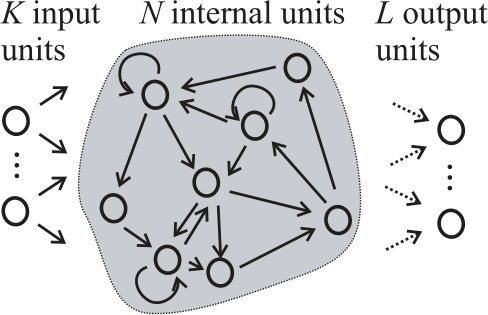
\includegraphics[scale = 0.5]{architecture}
\centering
\caption{Architecture of a network with K input units, N internal units and L output units (graphics 
taken from \cite{jaeg7}).}
\end{figure}

In this project we are using the version of ESNs with leaky integration as described in \cite{jaeg8}. 
Using this particular type of the network the activation of internal units follows the equation:
\begin{equation}\label{esn:1}
\mathbf{x}(n+1) = (1-\alpha)\mathbf{x}(n) +  \alpha\mathbf{f}(\mathbf{Wx}(n) +\mathbf{W^{in}u}(n+1) + \mathbf{b_N})
\end{equation}
where $\mathbf{b_N}$ is a fixed random N dimensional bias vector, $\alpha$ is the leaking rate of the network and $\mathbf{f}=(f_1...f_N)$ are the internal unit's output functions. In our case we will be using $\mathbf{tanh}$ as this function. The output is updated according to the equation:
\begin{equation}\label{esn:2}
\mathbf{y}(n+1) = g(\mathbf{W^{out}}\mathbf{x}(n+1)) 
\end{equation}
where $\mathbf{g}$ is an output activation function. In our case we will be using the identity function so 
$\mathbf{g}$ will be ignored. 
\subsubsection*{Training ESNs}
In the stage of training, the network is driven by a given teacher input signal 
$\mathbf{u}(1),...,\mathbf{u}(n_{train})$ which yields a sequence $\mathbf{x}(1),...,\mathbf{x}(n_{train})$ of 
network states. The obtained network states are collected into a matrix $\mathbf{X}$ of size 
$N\times (n_{train}-n_0)$, where $n_{train}$ is the training length and $n_0$ is the washout time. 
Along the teacher input signal, a teacher output signal is provided. The desired outputs $\mathbf{y}(n)$ 
are sorted row-wise into a teacher output collection matrix $\mathbf{Y_t}$ of size $(n_{train}-n_0)\times L$ \cite{spedia}. 
Then the output weights $\mathbf{W^{out}}$ are trained using linear regression following the equation:
\begin{equation}\label{esn:3}
\mathbf{W^{out}=Y_tX^T(XX^T} + \gamma^2I)^{-1}
\end{equation}
where $\gamma^2$ is the regularization coefficient and $I$ is the identity matrix. 
After training the output weight by linear regression the network is ready for testing.
\subsubsection*{Achieving Echo States}
Under certain conditions, the activations state $\mathbf{x}(n)$ of a recurrent neural network are a function of 
the input history presented to the network \cite{jaeg6}. More precisely there exists an echo function $\mathbf{E}$, 
such that the activation state of the network is calculated as:
\begin{equation}
\mathbf{x}(n) = \mathbf{E}(...,\mathbf{u}(n-1),\mathbf{u}(n))
\end{equation}
We give here a proposition from \cite{jaeg6} which gives sufficient conditions for the existence and the 
non-existence of echo states.
\begin{prop}
Assume a sigmoid network with unit output functions $f_i=tanh$. Let the weight matrix $\mathbf{W}$ have its 
largest singular value $\sigma_{max} <1$. Then the network has echo states for all admissible inputs. 
Let the weight matrix have a spectral radius $|\lambda_{max}| > 1$, where the spectral radius denotes the \
eigenvalue of the weight matrix with the largest absolute value. Then this network has no echo states if 
$\mathbf{u}(n)=0$ is an admissible input sequence.
\end{prop}
Note that scaling the weight matrix $\mathbf{W}$ with a scalar $\alpha$ scales the spectral radius and the 
singular values accordingly. In practice it is enough to achieve echo states if we have a spectral radius 
marginally smaller than 1. This would be achieved by scaling the matrix $\mathbf{W}$ with $\beta/|\lambda_{max}|$ 
where $\beta$ is marginally smaller than 1.
\subsection{Support Vector Machines}\label{svms}
Support Vector Machines (SVMs) are a popular machine learning method for classification, regression 
and other learning tasks. The original SVM algorithm was invented by Vladimir N. Vapnik and Alexey Ya. 
Chervonenkis in 1963. The current standard version was initially proposed by Cortes and Vapnik in 1993 
and published in 1995 \cite{cortes1995support}. The following sections explain the SVM algorithm as presented 
in \cite{fletcher2009support,law2006simple,berwick2003idiot}.
\subsubsection*{Motivation behind SVMs}
The basic idea of the SVM algorithm is to find an optimal hyperplane for linearly separable data points.
Given linearly separable training data points $\mathbf{x}_i\in R^n,i=1,....,l$, where each $\mathbf{x}_i$
belongs in one of the two classes $\mathbf{y}_i=-1$ or $+1$, the SVM algorithm tries to find an optimal hyperplane
separating the two classes \cite{fletcher2009support}. This hyperplane can be defined formally as:
\begin{equation}
  \mathbf{w}\cdot\mathbf{x} + \mathbf{b} = 0
\end{equation} where $\mathbf{w}$ is a weight vector normal to the hyperplane and $\mathbf{b}$ is a bias vector.
Support vectors are the data points closest to this separating
hyperplane and the aim of the algorithm is to maximize the distance of the hyperplane to the support
vectors \cite{law2006simple}. This distance is called the margin of the separating hyperplane.

\begin{figure}[H]
  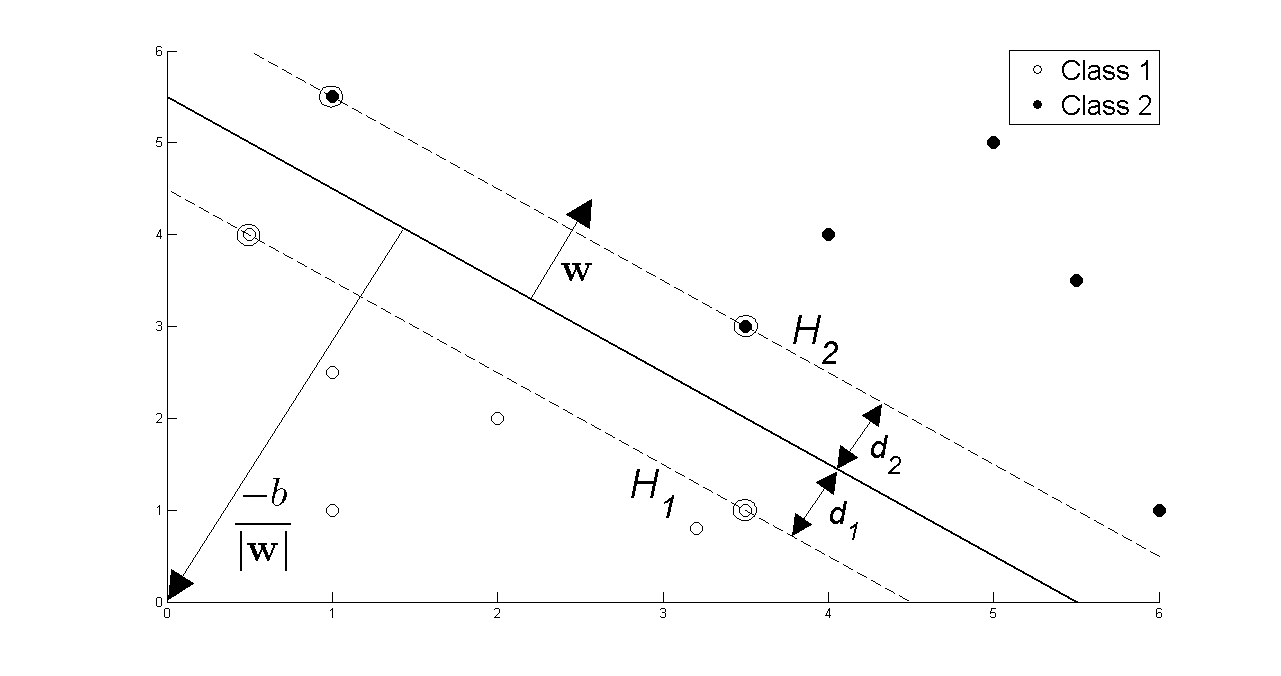
\includegraphics[scale=0.3]{hyperplane}
  \centering
  \caption{Hyperplane through two linearly separable classes (graphics taken from \cite{fletcher2009support}).}
\end{figure}
The figure above shows the optimal hyperplane through two linearly separable classes. 
$H_1$ and $H_2$ denote the planes on which the support vectors lie on. 
The margin of the hyperplane is $m = |d_1|+|d_2|$. Referring to this figure, implementing the SVM boils down to selecting
variables $\mathbf{w}$ and $\mathbf{b}$ such that:
\begin{equation}\label{svm1}
  \mathbf{x}_i\cdot\mathbf{w}+\mathbf{b}\geq +1 \quad \forall \mathbf{y}_i = +1
\end{equation}
\begin{equation}\label{svm2}
  \mathbf{x}_i\cdot\mathbf{w}+\mathbf{b}\leq -1 \quad \forall \mathbf{y}_i = -1
\end{equation}
The equations can be combined into:
\begin{equation}\label{svm3}
  \mathbf{y}_i(\mathbf{x}_i\cdot\mathbf{w}+\mathbf{b}) - 1 \geq 0 \quad \forall i
\end{equation}
As we said earlier the SVM algorithm aims to maximize the margin $m$. Simple vector geometry
shows that $m = \frac{2}{||\mathbf{w}||}$ \cite{fletcher2009support}. Maximizing $m$ is equivalent to minimizing
$\frac{1}{2}||\mathbf{w}||^2$, which leads to solving the following constrained optimization problem:
\begin{equation}\label{primal}
  min \ \frac{1}{2}||\mathbf{w}||^2 \quad s.t. \quad  \mathbf{y}_i(\mathbf{x}_i\cdot\mathbf{w}+\mathbf{b}) - 1 \geq 0 \quad \forall i
\end{equation}
The solution to this problem and the mathematical formalism behind it are documented in \cite{law2006simple}.
We ignore the step by step solution and present just the result. The original problem \ref{primal}, known as the primal problem,
is equivalent to the following dual problem \cite{law2006simple}:
\begin{equation}
  max \ W(\mathbf{\alpha}) = \sum_{i=1}^l \alpha_i - \frac{1}{2} \sum_{i=1,j=1}^l \alpha_i \alpha_j \mathbf{y}_i\mathbf{y}_j\mathbf{x}_i\mathbf{x}_j
  \quad s.t \quad \alpha_i \geq 0,\ \sum_{i=1}^l \alpha_i\mathbf{y}_i = 0
\end{equation}
This is a quadratic programming problem and a solution $\alpha=(\alpha_i)$ can be found using different approaches.
For SVM, sequential minimal optimization seems to be the most popular \cite{law2006simple}. A nice characteristic 
of the solution is that many of the $\alpha_i$ are $0$ and the $\mathbf{x}_i$ with non-zero $\alpha_i$ are the support 
vectors. Therefore we can construct $\mathbf{w}$ as a linear combination of a small number of data points \cite{law2006simple}:
\begin{equation}\label{svm4}
  \mathbf{w} = \sum_{j=1}^s \alpha_{t_j}\mathbf{y}_{t_j}\mathbf{x}_{t_j}
\end{equation}
where $t_j(j=1,...,s)$ are the indices of the $s$ support vectors.
After the optimal hyperplane is computed, the SVM classifier can categorize new data $\mathbf{z}$ by looking at the sign of the expression:
\begin{equation}
  f = \mathbf{w}\cdot\mathbf{z}+\mathbf{b}
\end{equation} and categorize it as class $1$ if the $f$ is positive and class $-1$ otherwise.
\subsubsection*{Extension to non-linearly Separable Data}
In order to extend the SVM methodology to handle data that is not fully linearly separable, we relax 
the constraints \ref{svm1} and \ref{svm2} to allow for misclassified points \cite{fletcher2009support}. This is done by introducing
positive slack variables $\xi_i$, $i=1,....,l$ and the new equations can be combined into:
\begin{equation}
  \mathbf{y}_i(\mathbf{x}_i\cdot\mathbf{w}+\mathbf{b}) - 1 + \xi_i\geq 0 \quad \text{where} \quad \xi_i\geq 0\ \forall i
\end{equation}
\begin{figure}[H]
  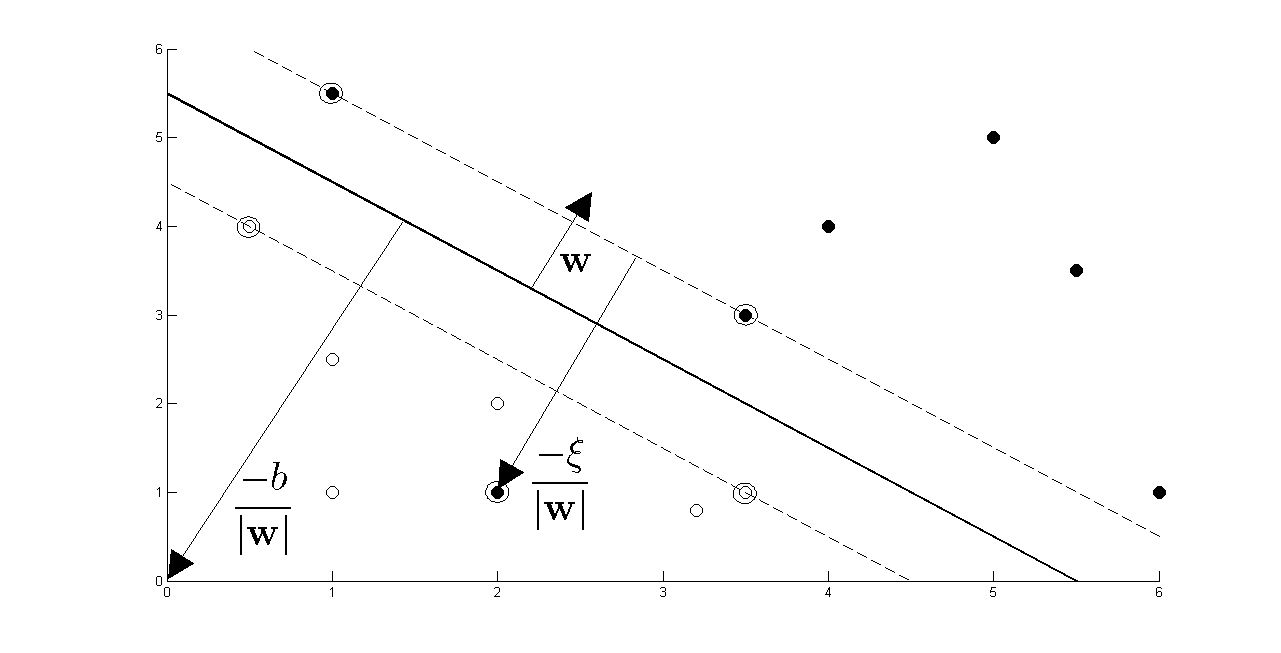
\includegraphics[scale=0.3]{nonlinear}
  \centering
  \caption{Hyperplane through two non-linearly separable classes (graphics taken from \cite{fletcher2009support}).}
\end{figure}
In this SVM version, data points on the incorrect side of the margin boundary have a penalty that increases with the distance
from it. The correctly classified data points have $\xi_i=0$. As we are trying to reduce the number of misclassifications,
we adapt the previous objective function \ref{primal} in the following way:
\begin{equation}
  min \ \frac{1}{2}||\mathbf{w}||^2+C\sum_{i=1}^l\xi_i\quad s.t. \quad \mathbf{y}_i(\mathbf{x}_i\cdot\mathbf{w}+\mathbf{b}) - 1 + \xi_i\geq 0 \ \forall i
\end{equation}
where the parameter $C$ controls the trade-off between the slack variable penalty and the size of the margin.
The new constrained optimization problem can be solved in the same way as in the linear separable case, except
there is an upper bound $C$ on $\alpha_i$ now \cite{law2006simple}. The dual problem in this case is:
\begin{equation}
  max \ W(\mathbf{\alpha}) = \sum_{i=1}^l \alpha_i - \frac{1}{2} \sum_{i=1,j=1}^l \alpha_i \alpha_j \mathbf{y}_i\mathbf{y}_j\mathbf{x}_i\mathbf{x}_j
  \quad s.t \quad C\geq\alpha_i \geq 0,\ \sum_{i=1}^l \alpha_i\mathbf{y}_i = 0
\end{equation}
The weight vector $\mathbf{w}$ can be constructed in the same way as in the linearly separable case.
\subsubsection*{Extension to non-linear Decision Boundary}
Many datasets cannot be separated by a linear hyperplane. The idea is to transform these data points
into a higher dimensional feature space which is linearly separable. After the transformation, the SVM algorithm can be applied to the transformed data points.
Computation in this new space can be quite costly but this is not a problem for the SVM, since we only calculate the inner product 
of the data points. As long as we can calculate the inner product in the feature space, we do not need the mapping explicitly \cite{law2006simple}.
This is the so called kernel trick. We define the kernel function $K$:
\begin{equation}
  K(\mathbf{x}_i,\mathbf{x}_j) = \phi(\mathbf{x}_i)\phi(\mathbf{x}_j)
\end{equation} where $\phi(\mathbf{x})$ is a map which transforms the data points into the linearly separable feature space.
For the linear decision boundary case, $\phi$ is the identity function. The dual problem in the case of non-linearly decision boundary
transforms to:
\begin{equation}\label{svm5}
  max \ W(\mathbf{\alpha}) = \sum_{i=1}^l \alpha_i - \frac{1}{2} \sum_{i=1,j=1}^l \alpha_i \alpha_j \mathbf{y}_i\mathbf{y}_jK(\mathbf{x}_i,\mathbf{x}_j)
  \quad s.t \quad C\geq\alpha_i \geq 0,\ \sum_{i=1}^l \alpha_i\mathbf{y}_i = 0
\end{equation}
The new data $\mathbf{z}$ can be categorized by looking at the sign of the expression:
\begin{equation}\label{svm6}
  f = \mathbf{w}\mathbf{\phi(z)}+\mathbf{b} = \sum_{j=1}^s \alpha_{t_j}\mathbf{y}_{t_j}K(\mathbf{x}_{t_j},\mathbf{z})+\mathbf{b} 
\end{equation} where $t_j$ is defined as in \ref{svm4}.
The kernel function, being an inner product, can be viewed as measure of similarity between two data points.
We present here 3 popular examples of kernel functions:
\begin{itemize}
  \item Polynomial kernel function with degree $d$:
  \begin{math}
    K(\mathbf{x},\mathbf{y}) = (\mathbf{x}\mathbf{y} + 1)^d
  \end{math}
  \item Radial basis function with width $\psi$:
  \begin{math}
    K(\mathbf{x},\mathbf{y}) = e^{\frac{-||\mathbf{x}-\mathbf{y}||^2}{2\psi^2}}
  \end{math}
  \item Sigmoid function with parameters $\kappa$ and $\theta$: 
  \begin{math}
    K(\mathbf{x},\mathbf{y}) = tanh(\kappa \mathbf{x} \mathbf{y}+\theta)
  \end{math}
\end{itemize}

In conclusion, training a SVM includes selecting a kernel function, choosing the kernel parameters and the value of $C$ and
solving a quadratic programming problem.
\subsubsection*{Multi-class Classification}
By their design SVMs are binary classifiers. To support multi-class classification, we use a so called one-vs.-one strategy.
If $k$ is the number of classes, $\frac{k(k-1)}{2}$ SVMs are constructed as described above and each one of them 
trains data from two classes solving the quadratic programming problem \ref{svm5}. For classification a voting strategy is used. Each binary classifier casts a vote
as described in \ref{svm6}
and in the end the class with the most votes is chosen as the predicted class. In case that two or more classes have identical votes, 
a random choice is made between these classes.
\subsubsection*{Estimating Probabilities}
The SVM algorithm predicts only class labels without probability information. Because we aim to apply an ensemble
learning approach, we need to extend the SVM algorithm to give probability estimates. We are using LIBSVM \cite{chang2011libsvm} for 
constructing the SVM classifier. Based on their implementation the probability weights for multi-class classification 
are estimated as follows:

Given $k$ classes of data, for any $\mathbf{x}$, pairwise class probabilities are estimated first based on \cite{lin2007note}:
\begin{equation*}
  r_{ij} = P(\mathbf{y}=i|\mathbf{y}=i\ or \ j,\mathbf{x})
\end{equation*}
If $u$ is the decision value at $\mathbf{x}$, we estimate $r_{ij}$ by the equation:
\begin{equation}\label{log}
  r_{ij} = \frac{1}{1+e^{Au+B}}
\end{equation}
where $A$ and $B$ are estimated by minimizing the negative log likelihood of training data. It has been observed that
decision values from training might overfit the model \ref{log}, so a five-fold cross-validation scheme is conducted to obtain
the decision values before estimating $A$ and $B$. After collecting all $r_{ij}$ values, the following optimization
problem is solved as proposed by \cite{wu2004probability}:
\begin{equation}\label{prob}
  \underset{\mathbf{P}}{min} \ \ \frac{1}{2}\sum_{i=1}^k \sum_{j:j\neq i}(r_{ji}p_i-r_{ij}p_j)^2
  \quad subject \ to \quad \forall i \ p_i\geq 0 ,\quad \sum_{i=1}^k p_i = 1 
\end{equation} 
After solving this optimization problem, the SVM can give probability estimates $p_i$ for each class.
A summary of the algorithm to solve the problem \ref{prob} is documented on \cite{chang2011libsvm} while 
more details are presented on \cite{wu2004probability}.
\subsection{Logistic Regression}\label{logistic}
We present in this section a summary of the logistic regression model as described in \cite{hosmer2013applied}.
Regression methods are a set of statistical processes for estimating the relationship between a response variable
and one or more explanatory variables. Logistic regression has become the standard model of analysis in the situation when the outcome of the response variable
is discrete. What distinguishes logistic regression from linear regression is that the outcome variable in logistic regression 
is dichotomous. 
\subsubsection*{Motivation behind Logistic Regression}
The logistic regression model is used to estimate the probability of a binary response based on ore more predictors.
We give first a definition of the logistic function. The logistic function $\sigma$ is a sigmoid function which takes a real input
and outputs a value between zero and one:
\begin{equation}
  \sigma(t) = \frac{1}{1+e^{-t}} = \frac{e^t}{1+e^t}
\end{equation}
Assume that we have $l$ training data points $(\mathbf{x}_i,\mathbf{y}_i)$ where
$\mathbf{x}_i \in R^n$ and $\mathbf{y}_i=1$ or $0$. The value of $\mathbf{y}\ 1$  means that a data point belongs to one 
class and the value $0$ denotes the membership to the other class. We can treat the membership to a certain class
as a dichotomous variable and use the logistic regression model to estimate the probability of the membership of a
data point $\mathbf{x}$ in the 'first' class:
\begin{equation}
  p(\mathbf{x}) = P(y=1|\mathbf{x}) = \sigma(g(\mathbf{x}))
\end{equation}
where $g$ is the inverse of the logistic function also called the logit function:
\begin{equation}
  g(\mathbf{x}) = ln(\frac{p(\mathbf{x})}{1-p(\mathbf{x})}) = \mathbf{w}_0+\mathbf{w}_1\mathbf{x}_1+.....+\mathbf{w}_n\mathbf{x}_n
\end{equation}
The assumption that $g(\mathbf{x})$ is a linear combination of coordinates of $\mathbf{x}$ comes from linear regression.
It remains for the logistic regression model to choose an optimal weight vector $\mathbf{w}\in R^{n+1}$. 

The method of estimation used in logistic regression is maximum likelihood. This method yields values for the unknown 
parameters which maximize the probability of obtaining the observed data. In order to apply this method we construct 
first the likelihood function as follows:
\begin{equation}
  l(\mathbf{w}) = \prod_{i=1}^l p(\mathbf{y}_i|\mathbf{x}_i) =  \prod_{i=1}^l p(\mathbf{x}_i)^{\mathbf{y}_i}(1-p(\mathbf{x}_i))^{1-\mathbf{y}_i}\quad .
\end{equation}
The principle of maximum likelihood is to select the estimate of $\mathbf{w}$ which maximizes the likelihood function.
However, it is easier mathematically to maximize the log of the likelihood function. This expression, known as log likelihood,
is defined as:
\begin{equation}\label{maxlg}
  L(\mathbf{w}) = \sum_{i=1}^l {\mathbf{y}_iln[p(\mathbf{x}_i)]+(1-\mathbf{y}_i)ln[1-p(\mathbf{x}_i)]}\quad .
\end{equation}
Maximizing the log likelihood require special mathematical software which is present in most statistical packages.
We do not present here an algorithm for maximizing \ref{maxlg} but such a solution is known to be found.
\subsubsection*{Classification}
Having found $\mathbf{w}$ that maximizes \ref{maxlg}, we can proceed to classifying testing data.
For a new data point $\mathbf{z}$, we calculate $p(\mathbf{z}) = \frac{1}{1+e^{-\mathbf{w}\mathbf{z}}}$.
If $p(\mathbf{z})\geq 0.5$, we classify $\mathbf{z}$ in the first class; otherwise $\mathbf{z}$ belongs to
the other class. Here we use the convention of letting $\mathbf{z}_0=1$, so that 
$\mathbf{wz} = \mathbf{w}_0 + \sum_{j=1}^n \mathbf{w}_j\mathbf{z}_j$.
\subsubsection*{$L_2$ Regularization}
To prevent overfitting, we use a $L_2$-regularized version of logistic regression. We are using LIBLINEAR \cite{fan2008liblinear}
for constructing the logistic regression model. Based on their implementation, the model solves the following optimization problem:
\begin{equation}\label{logfinal}
  \underset{\mathbf{w}}{min} \ \ \frac{1}{2}\mathbf{w}^2+C\sum_{i=1}^l\xi(\mathbf{w};\mathbf{x}_i;\mathbf{y}_i)
\end{equation}
where $\xi(\mathbf{w};\mathbf{x}_i;\mathbf{y}_i)$ is a loss function and $C\geq 0$ is the trade-off parameter
as in the SVM model. We should note here that the data is labeled differently with $\mathbf{y}_i \in \{-1,1\}$.
In this case, it is clear that we can assign $p(\mathbf{y}|\mathbf{x}) = p(\mathbf{y}\mathbf{x})$. 
As we said before the aim of the model is to maximize the log likelihood. As a loss function, this corresponds
to minimizing the negative of the log likelihood. We calculate in this way the loss function to be minimized:
\begin{equation}
  J(\mathbf{w}) = -ln(\prod_{i=1}^l p(\mathbf{y}_i|\mathbf{x}_i)) = - \sum_{i=1}^l ln(p(\mathbf{y}_i|\mathbf{x}_i))
  = \sum_{i=1}^l ln(\sigma(\mathbf{y}_i\mathbf{w}\mathbf{x}_i)^{-1}) = \sum_{i=1}^l ln(1+e^{-\mathbf{y}_i\mathbf{w}\mathbf{x}_i})
\end{equation}

which shows that $\xi(\mathbf{w};\mathbf{x}_i;\mathbf{y}_i) = ln(1+e^{-\mathbf{y}_i\mathbf{w}\mathbf{x}_i})$.
Problem \ref{logfinal} is solved by LIBLINEAR by implementing a trust region Newton method as described in \cite{lin2008trust}.
After finding the optimal solution $\mathbf{w}$ we classify new data $\mathbf{z}$ by looking at the sign of the
expression $\mathbf{w}\mathbf{z}$.
\subsubsection*{Multi-class Classification}
Logistic regression is a probabilistic binary classifier. To support multi-class classification, we use 
a so called one-vs.-rest strategy. If $k$ is the number of classes, $k$ binary models are fit (one for each class).
Each binary model solves the optimization problem \ref{logfinal} by treating samples of each class as the positive 
outcome and all the other samples as the negative outcome. For a testing data point $\mathbf{z}$, we calculate
the probability of the membership to each class. In the end the $k$ probability scores are normalized and the 
class with the highest probability is chosen as the predicted one. 
\subsection{Ensemble Learning}\label{voting}
Ensemble learning algorithms take a different approach from the classical machine learning algorithms.
Rather than constructing one best hypothesis to solve a certain problem, ensemble systems construct 
a set of hypotheses and combine these hypotheses to solve the original problem \cite{dietterich2002ensemble}.
Experimental evidence has shown that ensemble methods are often more accurate than any single hypothesis.
Learning algorithms that output only a single hypothesis might suffer from three problems that can be
partly overcome by ensemble methods \cite{dietterich2002ensemble}:
\begin{itemize}
  \item the statistical problem - This problem arises when the learning algorithm is searching a space 
  of hypotheses that is too large for the amount of available training data. In such cases, there may
  be several good hypotheses to be chosen from the hypothesis space. A simple vote of equally-good 
  classifiers can improve the performance of the model. A learning algorithm that suffers from this problem
  is said to have high "variance".
  \item the computational problem - The computational problem arises when the learning algorithm
  cannot guarantee to find the best hypothesis within the hypothesis space. For example, the procedure
  of training neural networks with gradient descent can get stuck in local minima. A weighted 
  combination of several different local minima can reduce the risk of choosing the wrong local minima 
  to output.
  \item the representation problem - This problem arises when the hypothesis space does not contain 
  any hypotheses that are good approximations of the true function $f$. By taking a weighted vote 
  of hypotheses, the learning algorithm may be able to form a more accurate approximation of $f$.
  A learning algorithm that suffers from this problem is said to have high "bias".
\end{itemize} 
Experimental measures have shown that ensemble methods can reduce both the variance and the bias
of learning algorithms \cite{dietterich2002ensemble}.

In the context of our problem, the ensemble system consists of 3 different classifiers (ESNs, SVMs, LR) 
which are trained individually to solve the problem of automatic music genre classification. 
Each of these classifiers predicts a $10$ dimensional probability vector for each song in the validation sets.
We combine these probability scores by a soft voting strategy. Assume that for a testing data point $\mathbf{z}$,
the three classifiers output respectively the three probability vectors $p_{\mathbf{z}_1},\ p_{\mathbf{z}_2},\ p_{\mathbf{z}_3}$.
We calculate a weighted sum of these probabilities:
\begin{equation}
  r_\mathbf{z} = \mathbf{w}_1p_{\mathbf{z}_1} + \mathbf{w}_2p_{\mathbf{z}_2} + \mathbf{w}_3p_{\mathbf{z}_3}
\end{equation}
where $r_\mathbf{z}$ denotes the final hypothesis for a data point $\mathbf{z}$. The predicted genre by the ensemble
system for $\mathbf{z}$ is the index of the highest value in $r_\mathbf{z}$. The weights $\mathbf{w}_1,\
\mathbf{w}_2,\ \mathbf{w}_3$ are also learned by a cross validation scheme.

\section{Documentation of Methods}
\subsection{Problem and Dataset Description}
The experiments are based on the famous standard dataset used by Tzanetakis and Cook \cite{tzan}.
This dataset consists of 1000 30s long audio files which have been annotated a genre. 
The audio files cover 10 different genres with 100 files per each genre. The ten represented genres
are: Blues, Classical, Country, Disco, Hip-hop, Jazz, Metal, Pop, Reggae and Rock.

Given this dataset, we aim to train three different classifiers and apply a 10-fold 
cross validation scheme to classify the dataset into the given genres. Performance of 
each classifier is analyzed. In the end we combine the three classifiers by a soft-voting 
strategy and analyze the performance of the ensemble. 
\subsection{State of the Art}
In our context, state of the art refers to the performance of the classifiers applied
on the dataset that we are using. The following table, taken from \cite{survey2}, compares the performance
of different algorithms using different type of features. The first results come from the creators
of the dataset who achieved up to 60\% classification accuracy. The most used classifier are
support vector machines. The MFCC feature set is used in almost every occasion. Most of the documented 
classifiers achieve mean classification accuracy in the range of 70-80\%.
\begin{figure}[H]
  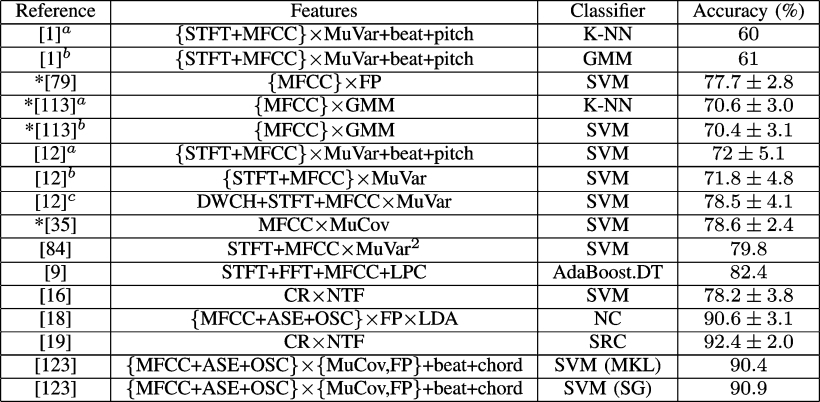
\includegraphics[scale=0.5]{art}
  \centering
  \caption{Performance comparison on the standard dataset}
\end{figure}
\subsection{Pre-processing}
The procedure of feature extraction differs for ESNs and the other two classifiers.
We feed continuous live data to the network while the features fed to the SVM and logistic regression
algorithm are 'global' features computed for the whole song. We document below the two different strategies
used in the pre-processing phase.
\begin{itemize}
  \item ESNs - For each audio file, the features described in \ref{exft} are computed for 
  each analysis window of 100ms long. We are calculating $20$ MFCCs, $20$ delta-cepstral
  coefficients and $8$ single features. After the feature extraction procedure, each audio file
  is represented as a matrix $\mathbf{A}$ of size $48\times f$, where $f$ is the number of frames
  of length 100ms for each audio file. 
  \item SVMs \& Logistic Regression - The extraction of 'global' features for these two classifiers 
  is based upon the above procedure for ESNs. We compute the mean and the variance of the $48$
  aforementioned features (calculated for each analysis window) over each texture window of 2s.
  Therefore, $96$ features are computed for each texture window. In the next step, the mean of these
  features is computed over the whole song segment, providing a global feature set of size $96$.
  In the end, we append to this feature set the covariance matrix of the $20$ MFCCs
  calculated over each analysis window. The usage of the covariance matrix of MFCCs led to better results
  using SVMs as a classifier \cite{ellis}. Finally, we have computed for each song a feature set of size $496$ which
  is fed to both the SVM and logistic regression algorithms.
\end{itemize}
\subsection{ESN Procedure}
The feature set fed to the network is of size $48$ so our network consists of $K=48$
input units. We are using the network to classify each musical piece into one of the 10 genres.
Therefore, the network will $L=10$ output units.
\subsubsection*{Constructing the Network}
Weight matrices $\mathbf{W^{in},\ W}$ and the bias vector $\mathbf{b_N}$ are randomly initialized with real numbers
in the interval $[-0.5,0.5]$. The spectral radius $\lambda_{max}$ of the weight matrix $\mathbf{W}$ is computed 
and we scale the matrix with the inverse of this factor. After this operation, $\mathbf{W}$ will have a spectral 
radius of 1.
\subsubsection*{Training the Network}
For each run, the network is trained using the state update equation \ref{esn:1}. For each musical piece, 
we ignore the first 30 frames from its matrix representation $\mathbf{A}$. Upon starting training a new musical 
piece the network state is initialized to $0$. The system states are collected in a matrix $\mathbf{X}$ of size 
$N\times (n_{train}-n_0)$. In our case $n_{train} = 900\cdot f$ and $n_0 = 900\cdot 30$, where $f$ is the number of 
frames for each musical piece. The output teacher matrix $\mathbf{Yt}$ will be of size $L\times (n_{train}-n_0)$. 
Each column vector of $\mathbf{Yt}$ consists of zeros and a $1$ on the right genre. By using the equation \ref{esn:3} 
the output weights matrix $\mathbf{W^{out}}$ is computed.
\subsubsection*{Testing the Network}\label{nettest}
Using state update equations \ref{esn:1} and \ref{esn:2}, the network is tested on each validation set.
For each musical piece in the validation set, the computed output vectors are saved in a matrix of size 
$L\times (f-30)$. The mean of this matrix over each row is computed resulting in a $L$ dimensional vector.
This vector is saved as the output of the network which is fed to the ensemble system.
The index of the highest value is chosen as the predicted genre. For each run we compute the classification accuracy
by dividing the number of correct predictions by 100. 
\subsection{SVM Procedure}\label{svmproc}
Each song is fed to the SVM algorithm as a pair $(x,y)$, where $\mathbf{x}$ is a feature set of size 496 
and $\mathbf{y}$ is a label from $1$ to $10$. For each validation round, the SVM is trained on 900 songs
as described in \ref{svms}. In the testing phase, we predict the genre for each of the 100 songs in the validation set.
The classification accuracy is computed for each run as in \ref{nettest}. Besides the class prediction, we compute
for each song probability vectors which will be fed to the ensemble system.
\subsection{Logistic Regression Procedure}\label{logproc}
Each song is fed to the logistic regression model as described in \ref{svmproc}. For each validation round, 
the model is trained on 900 songs as described in \ref{logistic}. In the testing phase, we compute a probability 
vector for each of the 100 songs in the validation set. This vector will be fed to the ensemble system. The class
with the highest probability is chosen as the predicted genre. The classification accuracy is computed for each run
as in \ref{nettest}.
\subsection{Ensemble Learning Procedure}
For each song in the validation set, we have computed three probability scores as explained in \ref{nettest},
\ref{svmproc}, \ref{logproc}.
We combine the probability scores by a soft voting strategy as documented in \ref{voting}. We compute accordingly
the classification accuracy for each run by dividing the number of correct predictions by 100.
\subsection{Cross Validation of Parameters}\label{cross}
A 10-fold cross validation is used to determine the parameters of the classifiers 
that achieve the best performance. The dataset is divided in 10 random smaller sets of 
100 audio files each. Each of these subsets is used iteratively as a validation set, while
the remaining data is used for training each of the classifiers. For each classifier configuration,
the mean classification accuracy over the 10 validation sets is computed and the configurations with 
the highest accuracy are chosen as the optimal ones. After the parameters of each classifier are 
decided, the weights of each classifier in the ensemble system are decided in the same fashion.
\begin{itemize}
  \item ESN Parameters - After allocating the initial weight matrices $\mathbf{W^{in}},\ \mathbf{W}$ and the bias factor $\mathbf{b_N}$, 
  it is for the best to scale these matrices respectively with scalars $\mathbf{s_1},\ \mathbf{s_2},\ \mathbf{s_3}$
  that improve the performance of the network. The reservoir size $N$, the leaking rate $\alpha$ and the regularization 
  coefficient $\gamma^2$ also affect the network behavior.
  \item SVM Parameters - The first choice for the SVM algorithm is that of the kernel function. After choosing the kernel function,
  we choose the kernel parameters (if any) and lastly the trade-off parameter $C$.
  \item LR Parameters - The only choice for the logistic regression model is that of the trade-off parameter $C$.
\end{itemize}
\section{Results of the Experiment}
\subsection{Optimal Parameters}
After performing a 10-fold cross validation scheme as documented in \ref{cross}, we present the parameters of the system
that give the best performance.
\subsubsection*{ESN Parameters}
\begin{itemize}
  \item $N = 800$
  \item $\alpha = 0.08$
  \item $\gamma^2 \in [0.0001,0.01]$
  \item $\mathbf{s_1}\in [0.95,1.1]$
  \item $\mathbf{s_2}\in [1.2,1.5]$
  \item $\mathbf{s_3}\in [0.1,0.2]$
  \item $n_0^* = 30$ (washout time for each musical piece)
\end{itemize}
\subsubsection*{SVM Parameters}
\begin{itemize}
  \item Kernel function - We chose a radial basis kernel function $K$ with width $\psi$:
  
  \begin{math}
    K(\mathbf{x},\mathbf{y}) = e^{\frac{-||\mathbf{x}-\mathbf{y}||^2}{2\psi^2}}
  \end{math}
    \item Kernel parameters - The only parameter of the kernel $\psi$, was set to its default value
    $\psi = \sqrt{\frac{N}{2}}$, where $N = 496$ is the number of features fed to the SVM.
    \item $C = 1000$
\end{itemize}
\subsubsection*{LR Parameters} $C = 1000$
\subsubsection*{Ensemble System Parameters}
$\mathbf{w}_1 = 7,\ \mathbf{w}_2 = 5,\ \mathbf{w}_3 = 2$
\subsection{Results}
\section{Conclusions}
\subsection{Future Work}
\nocite{*}
\newpage
\bibliographystyle{unsrt}
\bibliography{bsc-sample}

\end{document}
